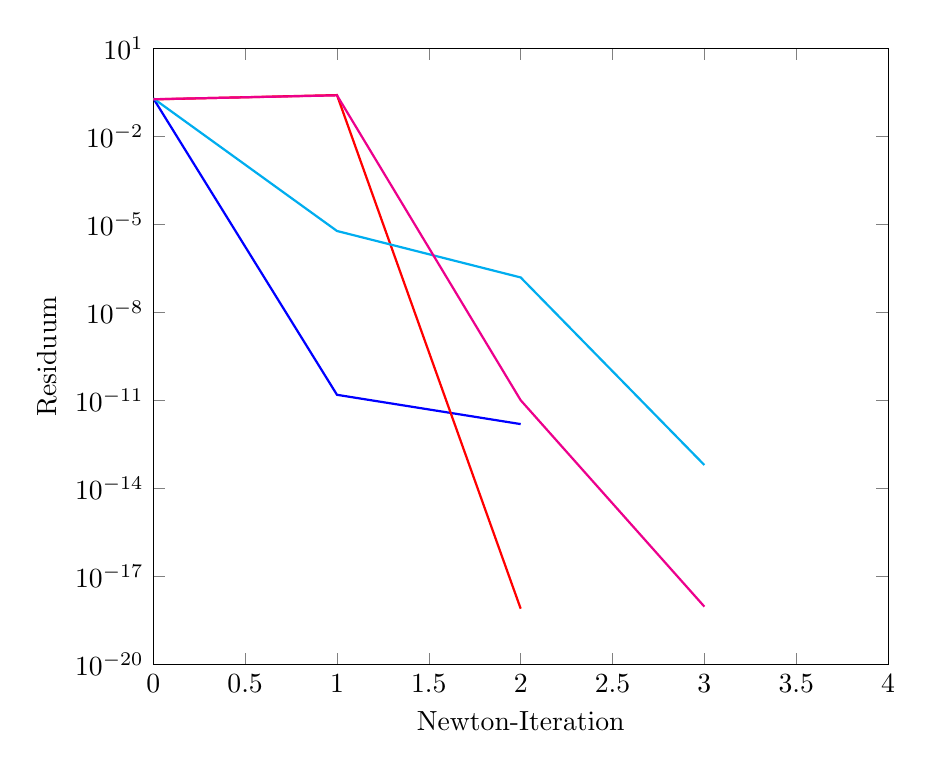
\begin{tikzpicture}[every plot/.append style={thick}] 
\begin{axis}[ 
label style={font=\normalsize}, 
xlabel={Newton-Iteration}, 
ylabel={Residuum}, 
xmin=0, xmax=4, 
ymode=log, 
ymin=0, ymax=10, 
width=0.9\textwidth, 
grid style=dashed, 
] 
\addplot[ 
color=blue, 
] 
coordinates { 
(0, 1.95e-01)(1, 1.56e-11)(2, 1.57e-12)}; 
\addplot[ 
color=red, 
] 
coordinates { 
(0, 1.80e-01)(1, 2.52e-01)(2, 8.10e-19)}; 
\addplot[ 
color=cyan, 
] 
coordinates { 
(0, 1.95e-01)(1, 5.93e-06)(2, 1.55e-07)(3, 6.33e-14)}; 
\addplot[ 
color=magenta, 
] 
coordinates { 
(0, 1.82e-01)(1, 2.47e-01)(2, 1.02e-11)(3, 9.53e-19)}; 
\end{axis} 
\end{tikzpicture} 
